% Doctorado en Ingeniería
% Creado por: Dr. Esteban Inga Ortega, PhD
% Universidad Politécnica Salesiana
% 20-Abril-2023
%=====================================================
%\documentclass[spanish,es-tabla,ansinew,12pt]{article}
\documentclass[12pt,a4paper]{article}
\usepackage{booktabs}
\usepackage[table,xcdraw]{xcolor}
\usepackage{lmodern}
\usepackage[centertags]{amsmath}
\usepackage[utf8]{inputenc}
\usepackage[T1]{fontenc}
\usepackage[mathscr]{eucal}
\usepackage{ifthen,calc,enumerate}
\usepackage{color}
\usepackage{array}
\usepackage{amsfonts}
\usepackage{textcomp}
\usepackage{amssymb}
\usepackage{amsthm}
\usepackage{newlfont}
\usepackage{graphicx}
\usepackage{subfigure}
\usepackage[hyperindex,colorlinks,breaklinks,pdfstartview=FitH,citecolor=cyan,linkcolor=blue,anchorcolor = green,citecolor=cyan,urlcolor  = blue]{hyperref}
%\usepackage[nonumberlist, numberedsection=true]{glossaries}
\usepackage{rotating}
\usepackage{lscape}
\usepackage{fancyhdr}
\usepackage{colortbl} %color para las tablas
\usepackage{float}
\usepackage{multirow}
\usepackage{enumerate} 
\usepackage{tikz}
\usepackage{url}
\usepackage{pgfplots}
\pgfplotsset{compat=1.18}
\usepackage[upright]{fourier} 
\usetikzlibrary{shapes}
\graphicspath{{Figuras/}}
\usepackage{verbatim}
\usepackage{tikz}
\usetikzlibrary{arrows.meta}
\tikzset{%
  >={Latex[width=2mm,length=2mm]},
  % Specifications for style of nodes:
            base/.style = {rectangle, rounded corners, draw=black,
                           minimum width=4cm, minimum height=1cm,
                           text centered, font=\sffamily},
  activityStarts/.style = {base, fill=blue!30},
       startstop/.style = {base, fill=red!30},
    activityRuns/.style = {base, fill=green!30},
         process/.style = {base, minimum width=2.5cm, fill=orange!15,
                           font=\ttfamily},
}
\usepackage{geometry}
\geometry{
    letterpaper,
    left=3cm,
    right=2.5cm,
    top=2.5cm,
    bottom=2.5cm
}
\renewcommand{\figurename}{Figura}
\renewcommand{\tablename}{Tabla}
\def\refname{Referencias}
%=====================================================
\begin{document}
%----------------------------------------------------------------------
%pat_definiciones
\newcommand\patTitulo
    {Arquetipos de datos semánticos en el diseño UX-UI y modelado del software: mejorando la usabilidad y eficiencia del sistema informático}
\newcommand\patTituloMayus
    {{\textsc \patTitulo}}
\newcommand\patNombre
    {Patricio Michael Paccha Angamarca}
\newcommand\patKeywords
    {Arquetipos de datos semánticos, diseño UX-UI, modelado de software, patrón de diseño de software}
\newcommand\patKeywordsIngles
    {Semantic data archetypes, UX-UI design, Software modeling, Software design pattern}

%portada
     \pagenumbering{arabic}
     \thispagestyle{empty}%
 \begin{titlepage}
    \begin{center}

{{\Large{\textsc{Universidad Politécnica Salesiana}}}} \rule[0.1cm]{16cm}{0.1mm}
\rule[0.5cm]{16cm}{0.6mm}
{\Large{\bf 
    DOCTORADO EN CIENCIAS COMPUTACIONALES 
}}
\end{center}
\vspace{15mm}
\begin{center}
{\LARGE{\bf 
    \patTituloMayus
}}\\
\vspace{6mm}
\end{center}
\vspace{22mm}
\par
\noindent

\begin{figure}
\begin{center}

\includegraphics[scale=0.3]{logoups.png}
\vspace{-0.2cm} 
\end{center}
\end{figure}


\begin{minipage}[t]{0.57\textwidth}
{\large{\bf Director:\\
    Ing. Esteban Inga, Ph.D. \\
{\vskip 5mm} Elaborado por:\\
    \patNombre
}}
\end{minipage}
\hfill
% \begin{minipage}[t]{0.47\textwidth}\raggedleft
%{\large{\bf Elaborado por:\\
%Nombre1 Nombre2 Apellido1 Apellido2}}
%\end{minipage}
\vspace{10mm}
\begin{center}
{\large{\bf 
    Fecha\\
    Julio, 2023 }}%inserire l'anno accademico de la inscritti
\end{center}
\end{titlepage}
%----------------------------------------------------------------------
\newpage
 \thispagestyle{empty}%
     \begin{center}
        \hyphenpenalty=10000\large\uppercase\expandafter{\textbf{
            \patTitulo
        }}
     \end{center}

     \begin{center}
         \vskip2cm
         \hyphenpenalty=10000\large\expandafter{\textbf{
            \patNombre
         }}  \\
         \vfill
         \normalsize 
            Trabajo de inicio de carrera para acceder al Doctorado en Ciencias Computacionales\\
         %\normalsize Mención en Sistemas Eléctricos de Potencia \\
         \vskip1cm
         \normalsize Director\\
         \vskip0.3cm
         \normalsize Ing. Esteban Inga, Ph.D. \\
     \end{center}
     \vfill
    \begin{center}
        
\includegraphics[width=6cm]{logoups.png}\\
        \uppercase\expandafter{Universidad Politécnica Salesiana} \\
        \uppercase\expandafter{DOCTORADO EN CIENCIAS COMPUTACIONALES} \\
        \uppercase\expandafter{Posgrados} \\
        \uppercase\expandafter{Quito, Ecuador} \\
        \uppercase\expandafter{2023}
    \end{center}
%=====================================================
\section{Información General}\label{sec:GeneralInformation}
%=====================================================
\begin{table*}[ht!]
\centering
\begin{tabular}{p{4cm}|p{9cm}}
\hline
\textbf{Título}  & 
Arquetipo de datos semánticos en el diseño UX-UI para el modelado de sistemas informáticos: mejora de la usabilidad y la eficiencia en el desarrollo de sistemas   \\
\hline
\textbf{Líder} & Nombre1 Nombre2 Apellido1 Apellido2 \\
\hline
\textbf{Unidad Académica} & Doctorado en Ciencias Computacionales \\
\hline
\multirow{2}{4cm}{\textbf{Entidades Involucradas}} & Universidad Politécnica Salesiana \\
& Movistar \\ \hline
\textbf{Lugar de Ejecución} & Quito, Universidad Politécnica Salesiana \\
\hline
\textbf{Fecha de Inicio} &   11-Oct-2023\\
\hline
\textbf{Fecha de Fin} &  11-Dic-2027 \\
\hline
\textbf{Keywords} & Wireless Sensor Networks, Rural coverage, Resource allocation, Optimization, Scheduling, Smart Cities \\
\hline
\end{tabular}
\end{table*}
%=====================================================
\section{Título del Proyecto}
%=====================================================
Optimización de redes inalámbricas mediante teoría de grafos y algoritmos de optimización combinatoria
%=====================================================
\section{Resumen}\label{sec:1}
%=====================================================
Text text text text text text text text text text text text text text text text text text text text text text text text text text text text text text text text text text text text text text text text text text text text text text text text text text text text text text text text text text text text text text text text text text text text text text text text text text text text text text text text text text text text text text text text text.

Text text text text text text text text text text text text text text text text text text text text text text text text text text text text text text text text text text text text text text text text text text text text text text text text text text text text text text text text text text text text text text text text text text text text text text text text text text text text text text text text text text text text text text text text text.

Text text text text text text text text text text text text text text text text text text text text text text text text text text text text text text text text text text text text text text text text text text text text text text text text text text text text text text text text text text text text text text text text text text text text text text text text text text text text text text text text text text text text text text text text text.

Text text text text text text text text text text text text text text text text text text text text text text text text text text text text text text text text text text text text text text text text text text text text text text text text text text text text text text text text text text text text text text text text text text text text text text text text text text text text text text text text text text text text text text text text text.
%=====================================================
\section{Descripción}\label{sec:Description}
%=====================================================
Text text text text text text text text text text text text text text text text text text text text text text text text text text text text text text text text text text text text text text text text text text text text text text text text text text text text text text text text text text text text text text text text text text text text text text text text text text text text text text text text text text text text text text text text text.

Text text text text text text text text text text text text text text text text text text text text text text text text text text text text text text text text text text text text text text text text text text text text text text text text text text text text text text text text text text text text text text text text text text text text text text text text text text text text text text text text text text text text text text text text text.

\begin{figure}[ht!]
\centering
{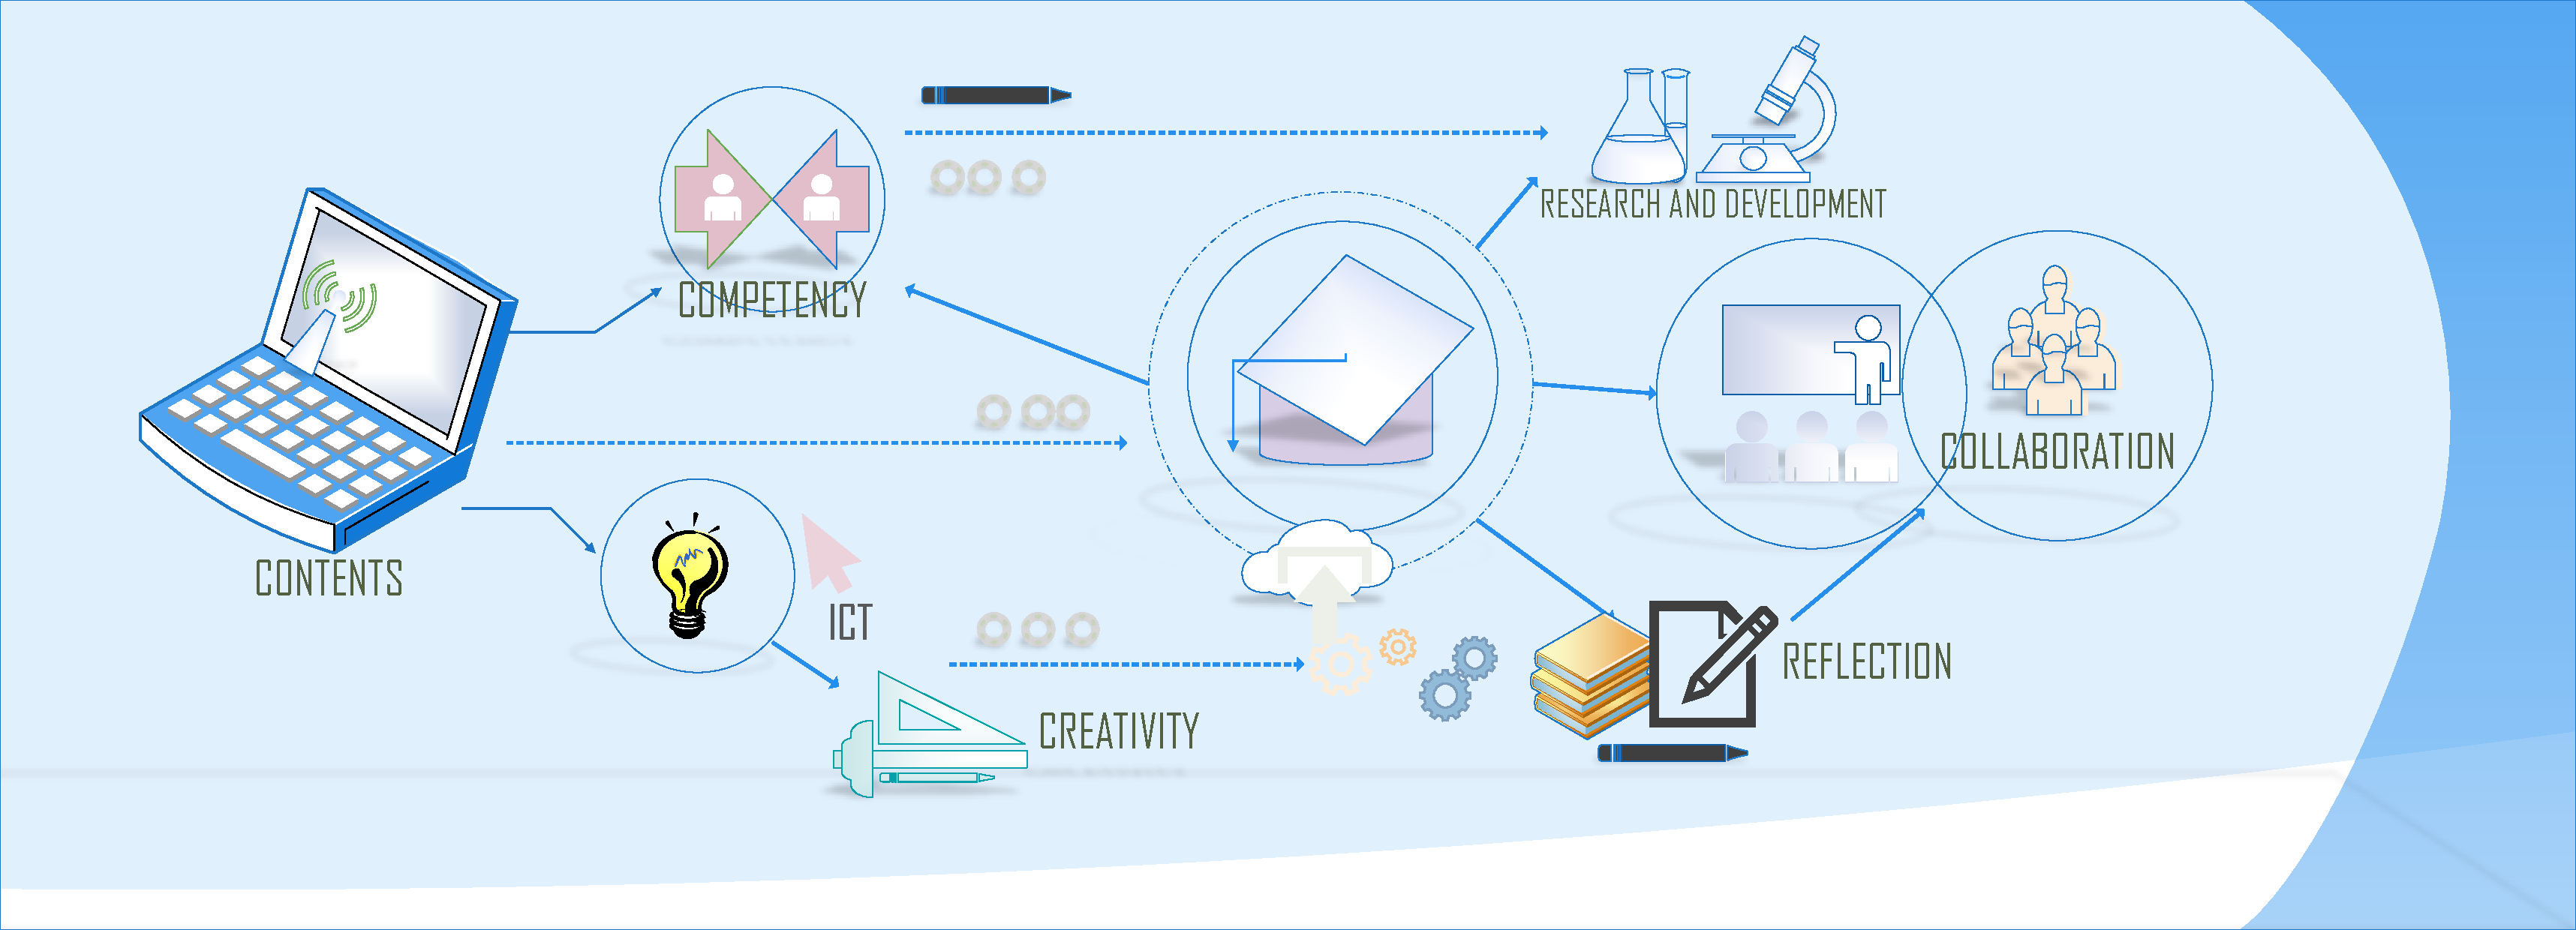
\includegraphics[clip=true,trim= 0cm 0cm 0cm 0cm, width=16cm]{Figuras/figure1.pdf}}
\caption{Esquema de optimización de redes inalámbricas utilizando teoría de grafos y algoritmos de optimización combinatoria}
\label{fig:0}
\end{figure}

\begin{figure}[H]
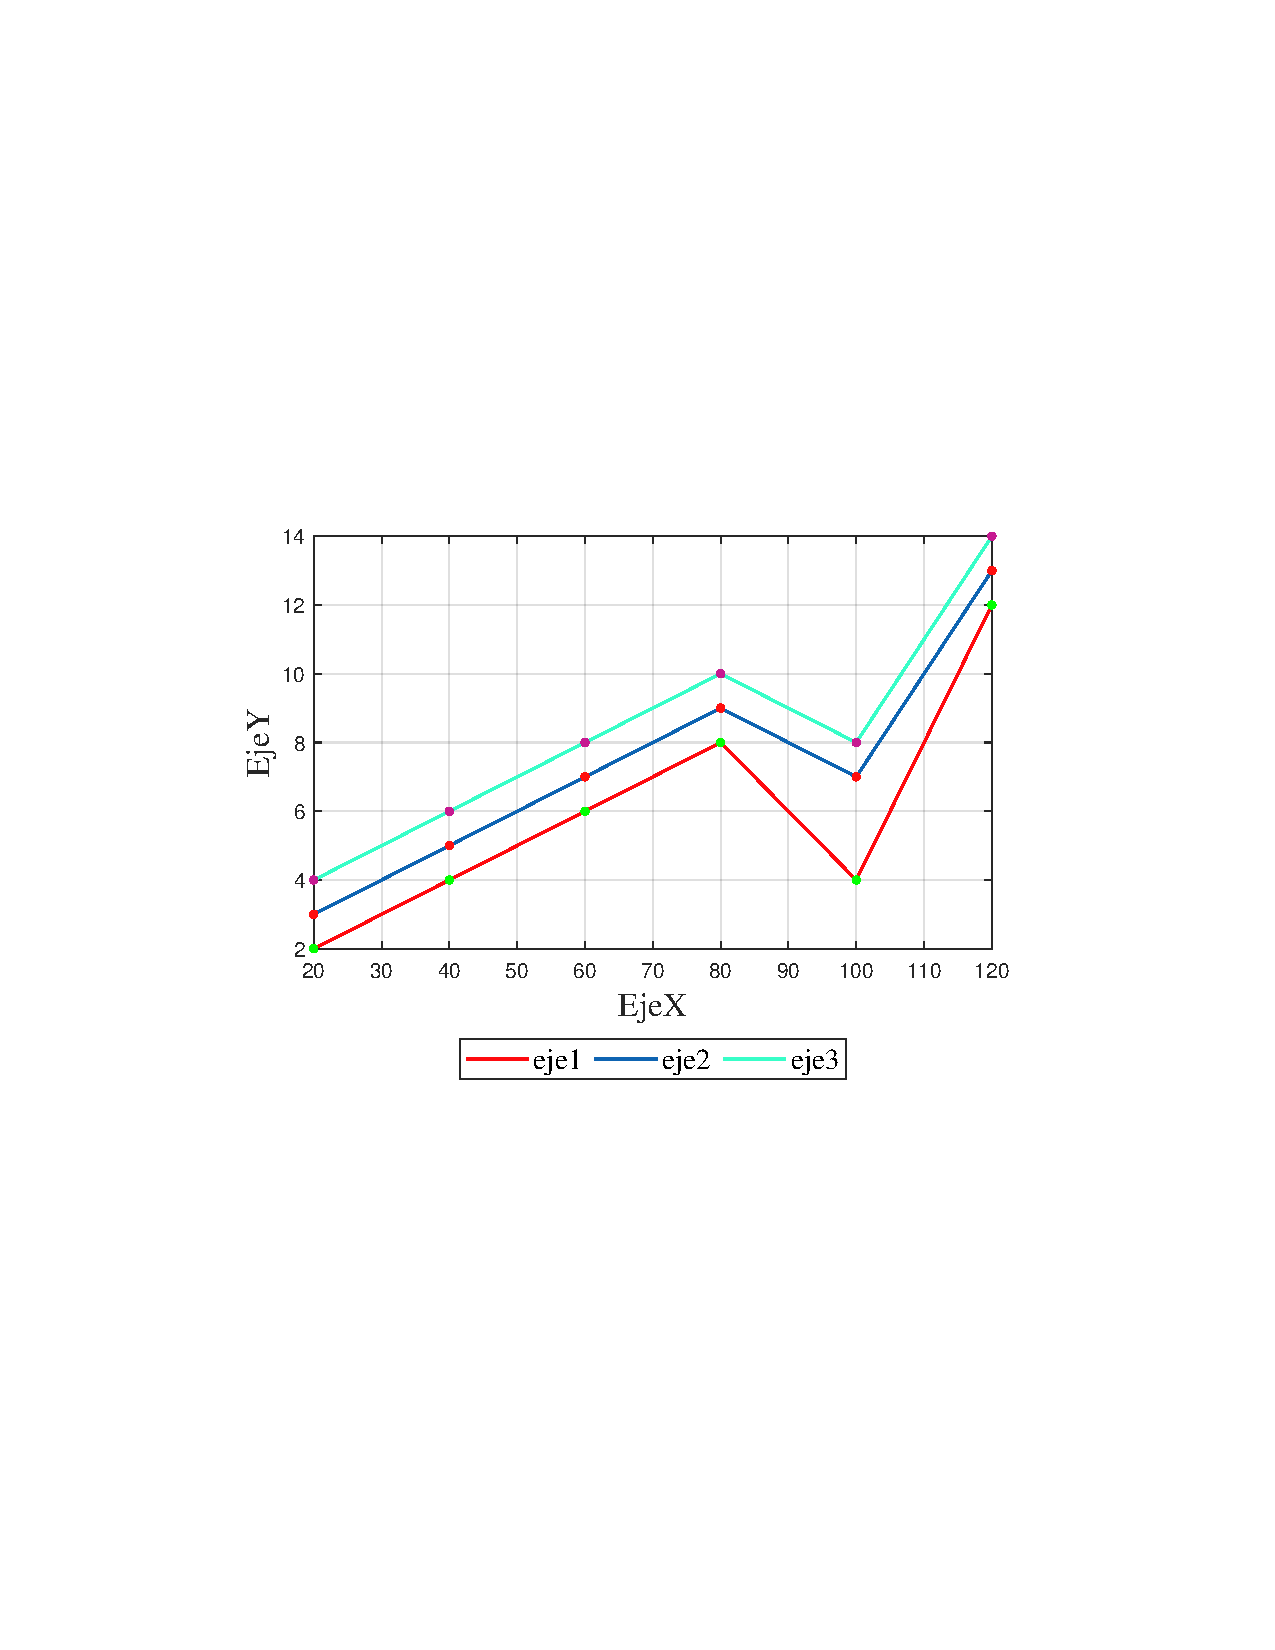
\includegraphics[clip=true,trim= 0cm 0cm 0cm 0cm,width=20cm]{Figuras/figureB.pdf}
\caption{Titulo de la figura}
\label{figB}
\end{figure}



%=====================================================
\subsection{Formulación del Problema}
\label{sec:2}
%=====================================================
Text text text text text text text text text text text text text text text text text text text text text text text text text text text text text text text text text text text text text text text text text text text text text text text text text text text text text text text text text text text text text text text text text text text text text text text text text text text text text text text text text text text text text text text text text \cite{Inga2023}.

Text text text text text text text text text text text text text text text text text text text text text text text text text text text text text text text text text text text text text text text text text text text text text text text text text text text text text text text text text text text text text text text text text text text text text text text text text text text text text text text text text text text text text text text text text \cite{Annersten2006}.


\begin{table}[H]
\centering
\caption{Espacio para el Titulo de la Tabla}
\label{tabB}
\begin{tabular}{llll}
Dato & Emergencia & Valor & Estado \\
\hline
23   & 120        & 36    & 28     \\
\hline
14   & 156        & 47    & 96     \\
\hline
12   & 45         & 67    & 90   \\
\hline
\end{tabular}
\end{table}


Text text text text text text text text text text text text text text text text text text text text text text text text text text text text text text text text text text text text text text text text text text text text text text text text text text text text text text text text text text text text text text text text text text text text text text text text text text text text text text text text text text text text text text text text text.

Text text text text text text text text text text text text text text text text text text text text text text text text text text text text text text text text text text text text text text text text text text text text text text text text text text text text text text text text text text text text text text text text text text text text text text text text text text text text text text text text text text text text text text text text text.
%=====================================================
\subsection{Hipótesis}
\label{sec:2a}
%=====================================================
Text text text text text text text text text text text text text text text text text text text text text text text text text text text text text text text text text text text text text text text text text text text text text text text text text text text text text text text text text text text text text text text text text text text text text text text text text text text text text text text text text text text text text text text text text


\begin{itemize}
  \item ......
  \item ......
\end{itemize}
%=====================================================
\subsection{Justificacion del problema}\label{sec:3}
%=====================================================
Text text text text text text text text text text text text text text text text text text text text text text text text text text text text text text text text text text text text text text text text text text text text text text text text text text text text text text text text text text text text text text text text text text text text text text text text text text text text text text text text text text text text text text text text text \cite{Garcia2023}.

Text text text text text text text text text text text text text text text text text text text text text text text text text text text text text text text text text text text text text text text text text text text text text text text text text text text text text text text text text text text text text text text text text text text text text text text text text text text text text text text text text text text text text text text text text.

Text text text text text text text text text text text text text text text text text text text text text text text text text text text text text text text text text text text text text text text text text text text text text text text text text text text text text text text text text text text text text text text text text text text text text text text text text text text text text text text text text text text text text text text text text.
Text text text text text text text text text text text text text text text text text text text text text text text text text text text text text text text text text text text text text text text text text text text text text text text text text text text text text text text text text text text text text text text text text text text text text text text text text text text text text text text text text text text text text text text text text.

%=====================================================
\subsection{Pertinencia}
\label{sec:4}
%=====================================================
Text text text text text text text text text text text text text text text text text text text text text text text text text text text text text text text text text text text text text text text text text text text text text text text text text text text text text text text text text text text text text text text text text text text text text text text text text text text text text text text text text text text text text text text text text.

Text text text text text text text text text text text text text text text text text text text text text text text text text text text text text text text text text text text text text text text text text text text text text text text text text text text text text text text text text text text text text text text text text text text text text text text text text text text text text text text text text text text text text text text text text.

Text text text text text text text text text text text text text text text text text text text text text text text text text text text text text text text text text text text text text text text text text text text text text text text text text text text text text text text text text text text text text text text text text text text text text text text text text text text text text text text text text text text text text text text text text.


%=====================================================
\section{Antecedentes}
\label{sec:5}
%=====================================================
Text text text text text text text text text text text text text text text text text text text text text text text text text text text text text text text text text text text text text text text text text text text text text text text text text text text text text text text text text text text text text text text text text text text text text text text text text text text text text text text text text text text text text text text text text.

Text text text text text text text text text text text text text text text text text text text text text text text text text text text text text text text text text text text text text text text text text text text text text text text text text text text text text text text text text text text text text text text text text text text text text text text text text text text text text text text text text text text text text text text text text.

Text text text text text text text text text text text text text text text text text text text text text text text text text text text text text text text text text text text text text text text text text text text text text text text text text text text text text text text text text text text text text text text text text text text text text text text text text text text text text text text text text text text text text text text text text.
%=====================================================
\subsection{Alcance del Proyecto}
\label{sec:6}
%=====================================================
Text text text text text text text text text text text text text text text text text text text text text text text text text text text text text text text text text text text text text text text text text text text text text text text text text text text text text text text text text text text text text text text text text text text text text text text text text text text text text text text text text text text text text text text text text.

Text text text text text text text text text text text text text text text text text text text text text text text text text text text text text text text text text text text text text text text text text text text text text text text text text text text text text text text text text text text text text text text text text text text text text text text text text text text text text text text text text text text text text text text text text.

\begin{itemize}
  \item text text text text text text text text text
  \item text text text text text text text text text
  \item text text text text text text text text text
\end{itemize}


%=====================================================
\subsection{Estado del Arte}
\label{sec:7}
%=====================================================
Text text text text text text text text text text text text text text text text text text text text text text text text text text text text text text text text text text text text text text text text text text text text text text text text text text text text text text text text text text text text text text text text text text text text text text text text text text text text text text text text text text text text text text text text text \cite{Inga2021}.

Text text text text text text text text text text text text text text text text text text text text text text text text text text text text text text text text text text text text text text text text text text text text text text text text text text text text text text text text text text text text text text text text text text text text text text text text text text text text text text text text text text text text text text text text text \cite{Inga2019}.

Text text text text text text text text text text text text text text text text text text text text text text text text text text text text text text text text text text text text text text text text text text text text text text text text text text text text text text text text text text text text text text text text text text text text text text text text text text text text text text text text text text text text text text text text text \cite{Inga2017}.


\begin{figure}[ht!]
\centering
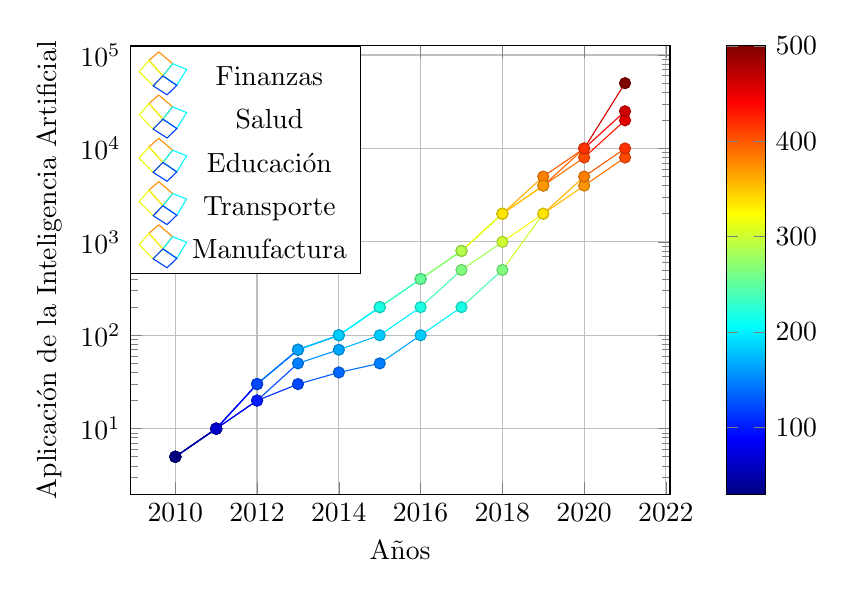
\begin{tikzpicture}
\begin{semilogyaxis}[
colormap/jet,
colorbar,
colorbar style={point meta min=30, point meta max=500, ytick={100,200,300,400,500}},
grid=major,
xlabel=Años,
ylabel=Aplicación de la Inteligencia Artificial,
domain=2010:2021,
x tick label style={/pgf/number format/1000 sep=},
legend style={at={(0,1)},anchor=north west},
]
\addplot+[mark=,solid,scatter,mesh,samples=12,scatter src=y] coordinates
{(2010,5) (2011,10) (2012,20) (2013,30) (2014,40) (2015,50) (2016,100) (2017,200) (2018,500) (2019,2000) (2020,4000) (2021,8000)};
\addplot+[mark=,solid,scatter,mesh,samples=12,scatter src=y] coordinates
{(2010,5) (2011,10) (2012,30) (2013,70) (2014,100) (2015,200) (2016,400) (2017,800) (2018,2000) (2019,4000) (2020,8000) (2021,20000)};
\addplot+[mark=*,solid,scatter,mesh,samples=12,scatter src=y] coordinates
{(2010,5) (2011,10) (2012,20) (2013,50) (2014,70) (2015,100) (2016,200) (2017,500) (2018,1000) (2019,2000) (2020,5000) (2021,10000)};

\addplot+[mark=*,solid,scatter,mesh,samples=12,scatter src=y] coordinates
{(2010,5) (2011,10) (2012,30) (2013,70) (2014,100) (2015,200) (2016,400) (2017,800) (2018,2000) (2019,5000) (2020,10000) (2021,25000)};

\addplot+[mark=*,solid,scatter,mesh,samples=12,scatter src=y] coordinates
{(2010,5) (2011,10) (2012,30) (2013,70) (2014,100) (2015,200) (2016,400) (2017,800) (2018,2000) (2019,4000) (2020,10000) (2021,50000)};
\legend{Finanzas, Salud, Educación, Transporte, Manufactura}
\end{semilogyaxis}
\end{tikzpicture}
\caption{Aumento de las aplicaciones de inteligencia artificial}
\label{fig:4}
\end{figure}

%=====================================================
\section{Objetivos}
\label{sec:8}
%=====================================================
Text text text text text text text text text text text text text text text text text text text text text text text text text text text text text text text text text text text text text text text text text text text text text text text text text text text text text text text text text text text text text text text text text text text text text text text text text text text text text text text text text text text text text text text text text.
%=====================================================
\subsection{Objetivo General}
\label{sec:9}
%=====================================================
Text text text text text text text text text text text  text text text text text text text text text text text text text text text text text text text text text text text.

%=====================================================
\subsection{Objetivos Específicos}
\label{sec:10}
%=====================================================


\begin{itemize}
  \item Text text text text text text text text text text text
  \item Text text text text text text text text text text text
  \item Text text text text text text text text text text text
\end{itemize}


%=====================================================
\section{Metodología}\label{sec:11}
%=====================================================
Text text text text text text text text text text text  text text text text text text text text text text text text text text text text text text text text text text text.

\begin{figure}[ht!]
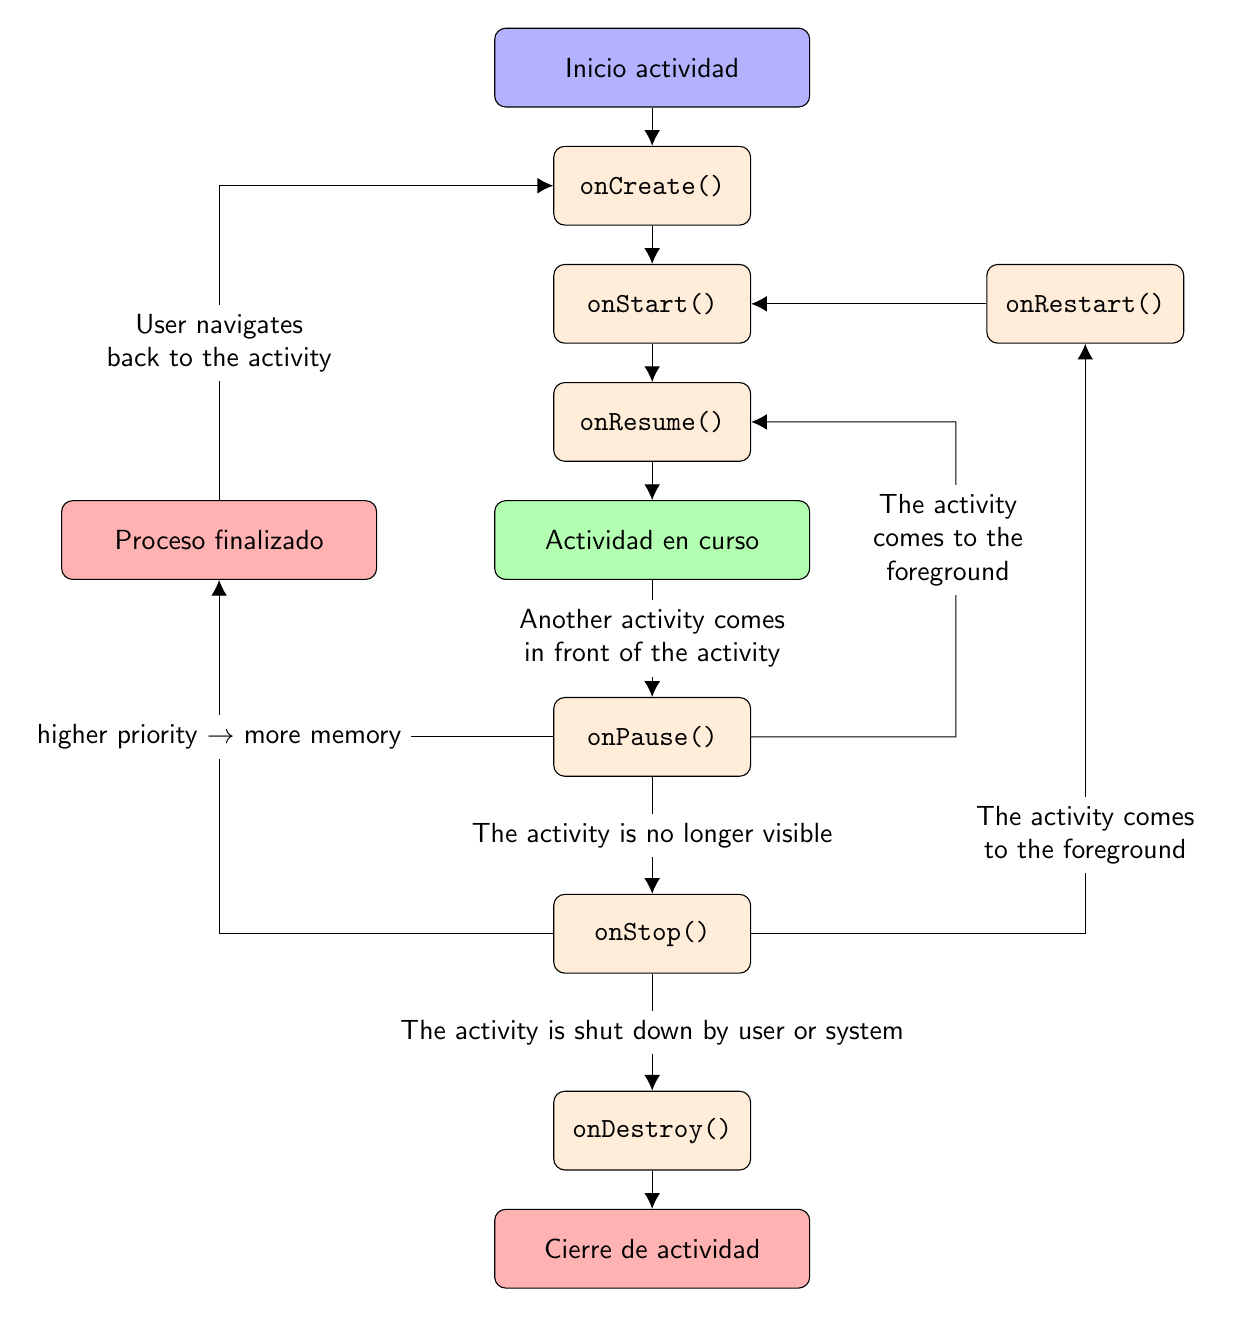
\begin{tikzpicture}[node distance=1.5cm,
    every node/.style={fill=white, font=\sffamily}, align=center]
  % Specification of nodes (position, etc.)
  \node (start)             [activityStarts]              {Inicio actividad};
  \node (onCreateBlock)     [process, below of=start]          {onCreate()};
  \node (onStartBlock)      [process, below of=onCreateBlock]   {onStart()};
  \node (onResumeBlock)     [process, below of=onStartBlock]   {onResume()};
  \node (activityRuns)      [activityRuns, below of=onResumeBlock]
                                                      {Actividad en curso};
  \node (onPauseBlock)      [process, below of=activityRuns, yshift=-1cm]
                                                                {onPause()};
  \node (onStopBlock)       [process, below of=onPauseBlock, yshift=-1cm]
                                                                 {onStop()};
  \node (onDestroyBlock)    [process, below of=onStopBlock, yshift=-1cm] 
                                                              {onDestroy()};
  \node (onRestartBlock)    [process, right of=onStartBlock, xshift=4cm]
                                                              {onRestart()};
  \node (ActivityEnds)      [startstop, left of=activityRuns, xshift=-4cm]
                                                        {Proceso finalizado};
  \node (ActivityDestroyed) [startstop, below of=onDestroyBlock]
                                                    {Cierre de actividad};     
  % Specification of lines between nodes specified above
  % with aditional nodes for description 
  \draw[->]             (start) -- (onCreateBlock);
  \draw[->]     (onCreateBlock) -- (onStartBlock);
  \draw[->]      (onStartBlock) -- (onResumeBlock);
  \draw[->]     (onResumeBlock) -- (activityRuns);
  \draw[->]      (activityRuns) -- node[text width=4cm]
                                   {Another activity comes in
                                    front of the activity} (onPauseBlock);
  \draw[->]      (onPauseBlock) -- node {The activity is no longer visible}
                                   (onStopBlock);
  \draw[->]       (onStopBlock) -- node {The activity is shut down by
                                   user or system} (onDestroyBlock);
  \draw[->]    (onRestartBlock) -- (onStartBlock);
  \draw[->]       (onStopBlock) -| node[yshift=1.25cm, text width=3cm]
                                   {The activity comes to the foreground}
                                   (onRestartBlock);
  \draw[->]    (onDestroyBlock) -- (ActivityDestroyed);
  \draw[->]      (onPauseBlock) -| node(priorityXMemory)
                                   {higher priority $\rightarrow$ more memory}
                                   (ActivityEnds);
  \draw           (onStopBlock) -| (priorityXMemory);
  \draw[->]     (ActivityEnds)  |- node [yshift=-2cm, text width=3.1cm]
                                    {User navigates back to the activity}
                                    (onCreateBlock);
  \draw[->] (onPauseBlock.east) -- ++(2.6,0) -- ++(0,2) -- ++(0,2) --                
     node[xshift=1.2cm,yshift=-1.5cm, text width=2.5cm]
     {The activity comes to the foreground}(onResumeBlock.east);
  \end{tikzpicture}
\caption{Metodología aplicada en la Investigación}
\label{fig2}
\end{figure}

Text text text text text text text text text text text  text text text text text text text text text text text text text text text text text text text text text text text.

Text text text text text text text text text text text  text text text text text text text text text text text text text text text text text text text text text text text.


%=====================================================
\section{Supervisión y Organización}
%=====================================================
Text text text text text text text text text text text  text text text text text text text text text text text text text text text text text text text text text text text.

%=====================================================
\section{Cronograma del Proyecto}
%=====================================================
Text text text text text text text text text text text  text text text text text text text text text text text text text text text text text text text text text text text.

Text text text text text text text text text text text  text text text text text text text text text text text text text text text text text text text text text text text.

\clearpage

\begin{table}[H]
\caption{Cronograma de Actividades}
\begin{center}
\begin{tabular}{|p{4.0cm}|c|c|c|c|c|c|c|c|c|c|c|c|c|c|c|c|}
\hline
Actividades &                  \multicolumn{ 4}{|c}{Primer Año} &                 \multicolumn{ 4}{|c}{Segundo Año} &                  \multicolumn{ 4}{|c}{Tercer Año} &                 \multicolumn{ 4}{|c|}{Cuarto Año} \\
\hline
 & $1$ & $2$ & $3$ & $4$ & $1$ & $2$ & $3$ & $4$ & $1$ & $2$ & $3$ & $4$ & $1$ & $2$ & $3$ & $4$ \\
\hline
\hline
\textbf{Actividades Generales}  &  &  &  &  &      &  &  &  &      &  &  &  &      &  &  &  \\ \hline
$~~$Estudios Iniciales    & $\blacksquare$ & $\blacksquare$ & $\blacksquare$ & $\blacksquare$ &      &  &  &  &      &  &  &  &      &  &  &  \\ \hline
$~~$Estado del Arte   &  &  &  &  &     $\blacksquare$ & $\blacksquare$ & $\blacksquare$ & $\blacksquare$ &      &  &  &  &      &  &  &  \\ \hline
$~~$Formulación del Problema   &  &  &  &  &      &  & $\blacksquare$ &  &      &  &  &  &      &  &  &  \\ \hline
$~~$Propuesta de Titulación   &  &  &  &  &      &  &  &  &      &  &  &  &     $\blacksquare$ &  &  &  \\ \hline
$~~$Escritura Trabajo de Titulación      &  &  &  &  &      &  &  &  &      &  &  &  &      & $\blacksquare$ &  &  \\ \hline
$~~$Presentación Oral      &  &  &  &  &      &  &  &  &      &  &  &  &      &  &  & $\blacksquare$ \\ \hline \hline

\textbf{Covertura Rural}      &  &  &  &  &      &  &  &  &      &  &  &  &      &  &  &  \\ \hline
$~~$Definición de Escenarios  &  &  &  &  &     $\blacksquare$ & $\blacksquare$ &  &  &      &  &  &  &      &  &  &  \\ \hline
$~~$Modelo de Despligue        &  &  &  &  &     $\blacksquare$ & $\blacksquare$ & $\blacksquare$ & $\blacksquare$ &      &  &  &  &      &  &  &  \\ \hline
$~~$Tests                    &  &  &  &  &      &  & $\blacksquare$ & $\blacksquare$ &     $\blacksquare$ &  &  &  &      &  &  &  \\ \hline
$~~$Campaña de Simulación     &  &  &  &  &      &  &  & $\blacksquare$ &     $\blacksquare$ &  &  &  &      &  &  &  \\ \hline
$~~$Analisis de Resultados      &  &  &  &  &      &  &  &  &      & $\blacksquare$ & $\blacksquare$ &  &      &  &  &  \\ \hline
$~~$Escritura de Paper        &  &  &  &  &      &  &  &  &      & $\blacksquare$ & $\blacksquare$ & $\blacksquare$ &     $\blacksquare$ &  &  &  \\ \hline \hline

\textbf{Asignación de Recursos} &  &  &  &  &      &  &  &  &      &  &  &  &      &  &  &  \\ \hline
$~~$Defición del Problema       &  &  &  &  &      &  &  &  &     $\blacksquare$ & $\blacksquare$ & $\blacksquare$ & $\blacksquare$ &      &  &  &  \\ \hline
$~~$Modelo de Despliegue        &  &  &  &  &      &  &  &  &      & $\blacksquare$ & $\blacksquare$ & $\blacksquare$ &      &  &  &  \\ \hline
$~~$Tests                    &  &  &  &  &      &  &  &  &      &  & $\blacksquare$ & $\blacksquare$ &      &  &  &  \\ \hline
$~~$Campaña de Simulación     &  &  &  &  &      &  &  &  &      &  &  & $\blacksquare$ &      &  &  &  \\ \hline
$~~$Analisis de Resultados      &  &  &  &  &      &  &  &  &      &  &  & $\blacksquare$ &     $\blacksquare$ &  &  &  \\ \hline
$~~$Escritura de Papers        &  &  &  &  &      &  &  &  &      &  &  & $\blacksquare$ &     $\blacksquare$ & $\blacksquare$ &  &  \\ \hline 
\end{tabular}
\end{center}
\end{table}
%=====================================================
\section{Resultados Previstos}
%=====================================================
Text text text text text text text text text text text  text text text text text text text text text text text text text text text text text text text text text text text.

Text text text text text text text text text text text  text text text text text text text text text text text text text text text text text text text text text text text.

Text text text text text text text text text text text  text text text text text text text text text text text text text text text text text text text text text text text.
%=====================================================
\section{Estrategias para Presentar Resultados}
%=====================================================
Text text text text text text text text text text text  text text text text text text text text text text text text text text text text text text text text text text text.

Text text text text text text text text text text text  text text text text text text text text text text text text text text text text text text text text text text text.
Text text text text text text text text text text text  text text text text text text text text text text text text text text text text text text text text text text text.

Text text text text text text text text text text text  text text text text text text text text text text text text text text text text text text text text text text text.
%=====================================================
\section{Sectores Beneficiados}
%=====================================================
Text text text text text text text text text text text  text text text text text text text text text text text text text text text text text text text text text text text.

Text text text text text text text text text text text  text text text text text text text text text text text text text text text text text text text text text text text.

Text text text text text text text text text text text  text text text text text text text text text text text text text text text text text text text text text text text.
%=====================================================
\section{Grupos de investigación}
%=====================================================
\subsection{Grupo Interno}

\textbf{GIREI - Grupo de Investigación en Redes Eléctricas Inteligentes}
\subsection{Grupo Externo}

\textbf{Movistar - Empresa Telefónica}. 
%=====================================================
\section{Presupuesto}
%=====================================================
Text text text text text text text text text text text  text text text text text text text text text text text text text text text text text text text text text text text.


\begin{table}[ht!]
\caption{Descripción del personal}
\begin{tabular}{|p{1.1cm}|p{1.1cm}|p{1.1cm}|p{1.1cm}|p{1.3cm}|p{1.1cm}|p{1.1cm}|p{1.1cm}|p{1.1cm}|p{1.1cm}|} \hline
Person. & Grado & Func. & Dedic.  & Dedic.  & \multicolumn{4}{|c|}{Recursos} & Total \\ \cline{6-9}
  &   &   & (horas / semana)  &  (\# Meses) & Est. PhD  & UPS & Emp. Privada & Senescyt &  \\ \hline \hline
Nombre1 Apellido1  & Ing  & Mst Estudiante  & 40 & 48 & - & - & - & 115.2M & 115.2M \\ \hline
Nombre2 Apellido2  & PhD  & Tutor & 4 & 48 & - & - & 57.6M & - & 57.6M \\ \hline
Total &    &   &   &   &   &   & 57.6M &  115.2M & 172.8M \\ \hline
\end{tabular}
\end{table}

%=====================================================
\begin{table}[ht!]
\caption{Descripción del equipo}
\begin{tabular}{|p{3.4cm}|p{3.4cm}|p{1.1cm}|p{1.1cm}|p{1.1cm}|p{1.1cm}|p{1.1cm}|} \hline
Equipos & Justificación & \multicolumn{4}{|c|}{Recursos} & Total \\ \cline{3-6}
 &   & Est. Mst & UPS & Emp. Privada & Senescyt &  \\ \hline \hline
Desktop PC 1 & Trabajo en UPS  & - & 4.0M & - & - & 4.0M \\ \hline
Personal Laptop & Trabajo General & 8.0M & - & - & - & 8.0M \\ \hline
Total &    & 8.0M & 4.0M & - & - & 12.0M \\ \hline
\end{tabular}
\end{table}

%=====================================================
\begin{table}[H]
\caption{Síntesis}
\begin{tabular}{|p{7.0cm}|p{1.1cm}|p{1.1cm}|p{1.1cm}|p{1.1cm}|p{1.1cm}|} \hline
Item & \multicolumn{4}{|c|}{Recursos} & Total \\ \cline{2-5}
  & Est. Mst. & UPS & Movistar & Senescyt &  \\ \hline \hline

Personal     & -    & -    & 57.6M & 115.2M & 172.8M \\ \hline
Equipamiento    & 8.0M & 4.0M & -     & -      & 12.0M \\ \hline
Materiales     & 3.0M & 1.0M & -     & -      & 4.0M \\ \hline
Software      & -    & 7.0M & -     & -      & 7.0M \\ \hline
Bibliografía  & 1.5M & 2.0M & -     & -      & 3.5M \\ \hline
Publicaciones  & 2.0M & 3.0M & -     & -      & 5.0M \\ \hline
Viajes         & 5.0M & 10.0M& -     & 22.0M  &37.0M \\ \hline
Trabajo de Grado        & -    & 7.0M & -     & -      & 7.0M \\ \hline
Total         &19.5M & 34.0M& 57.6M & 137.2M & 248.3M \\ \hline
\end{tabular}
\end{table}


%=====================================================
\section{Propiedad Intelectual}
%=====================================================
Los derechos de autor moral pertenecen al estudiante de doctorado y al asesor del proyecto y a cualquier persona que haga una contribución intelectual original, durante el proceso o en el resultado final del proyecto. El estudiante de doctorado y el asesor deben ser el autor y coautor de todas las publicaciones nacionales e internacionales generadas por el proyecto. La apariencia de otras personas depende de la calidad de la colaboración recibida. Los derechos de propiedad intelectual se asignan a la Universidad Politécnica Salesiana. 

\bibliographystyle{IEEEtran}

\bibliography{./Referencias}
\vfill
\end{document} 
